\documentclass[conference]{IEEEtran}
\usepackage[utf8]{inputenc}
\usepackage[german]{babel}

\usepackage{graphicx}
\graphicspath{figures/}

\makeatletter
\let\@copyrightspace\relax
\makeatother

\begin{document}

\title{MAC Authentication Bypass (MAB)\\ in Industrie 4.0}
\author{
	Umut-Vural Mitiler\\
	u.mitiler@stud.hs-wismar.de
	\and
	Fakultät für Ingenieurwissenschaften\\
	Hochschule Wismar\\
	Master IT-Sicherheit und Forensik\\
	Industrial Security\\
	Gruppe FFM-08
	\and
	David Schunke\\
	d.schunke@stud.hs-wismar.de
}

\maketitle

\thispagestyle{plain}
\pagestyle{plain}

%

\begin{abstract}
Eine kurze Beschreibung des Papers, worum gehts, was wird erklärt, was ist das Resultat.
\end{abstract}

%

\section{Einleitung}
Grundsätzliche Motviation für das Thema

\subsection{Industrie 4.0}
Beschreibung von Industrie 4.0, was bedeutet es, worum gehts

\subsection{Network Access Control}
Beschreibung was NAC ist, was ist die Motivation, was soll das Ganze

%

\section{Grundlagen}
Kurze technische Einführung

\subsection{dot1x}
Erklärung dot1x, was macht es, kurz technische Übersicht als Basis für MAB

\begin{figure}[hbt]
	\centering
	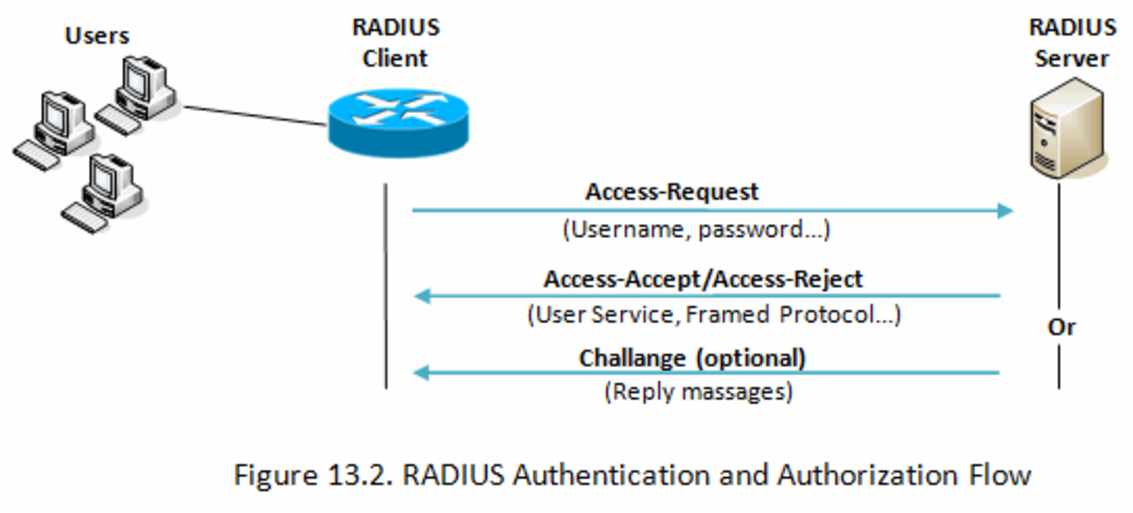
\includegraphics[width=8cm]{figures/Radius}
	\caption{Foobar \cite{einstein}}
\end{figure}

\subsection{Technische Umsetzung von MAB}
wie funktioniert MAB konkret, kurze technische Detailübersicht, was ist der Unterschied zu dot1x

%

\section{Praxiseinsatz}
NAC in der Praxis allgemein

\subsection{Heutiger Einsatz}
Wie wird MAB bereits jetzt eingesetzt\\
Fallback\\
Drucker, Telefone, IP-Phones, Kameras

\subsection{Relevanz in Industrie 4.0}
Hier kommt alles zur Relevanz von Industrie 4.0\\
Skalierbarkeit, Heterogene Landschaft, Einbindung von "Leichen"

%

\newpage

\section{Ergebnis}
Zusammenfassung was MAB macht, was es ist, wofür es nicht geeignet ist\\
Vorteile und Nutzen\\
Nachteile und Gefahren\\
Gegenmaßnahmen und Kombination mit anderen Technologien, wie z.B. IDS, usw.
\newline

Wie sieht die Zukunft von MAB aus

%

\bibliographystyle{IEEEtran}
\bibliography{references}

\end{document}